

\section{Preamble}
Open source software (OSS) repositories contain a large amount of data that has been accumulated along the software development process. Not only source code but also metadata available from different related sources, e.g. communication channels, bug tracking systems, is beneficial to the development process once it is properly mined. Research has been performed to understand and predict software evolution, exploiting the rich metadata available at OSS repositories. This allows for the reduction of effort in knowledge acquisition and quality gain. Developers can leverage the underlying knowledge if they are equipped with suitable tools. For instance, it is possible to empower IDEs by means of tools that continuously monitor the developer's activities and contexts in order to activate dedicated recommendation engines \cite{Ponzanelli:2014:MST:2597073.2597077}. 

%To aim for software quality, for developers it is necessary to understand how similar, mature projects are developed.   it is necessary

To aim for software quality, developers normally build their project by learning from mature OSS projects having comparable functionalities. To this end, the ability to search for similar software projects with respect to different criteria such as functionalities and dependencies plays an important role in the development process. Two projects are deemed to be similar if they implement some features being described by the same abstraction, even though they may contain various functionalities for different domains \cite{McMillan:2012:DSS:2337223.2337267}. Understanding the similarities between open source software projects allows for reusing of source code and prototyping, or choosing alternative implementations \cite{Schafer:2007:CFR:1768197.1768208},\cite{10.1109/SANER.2017.7884605}, thereby improving software quality. Meanwhile measuring the similarities between developers and software projects is a critical phase for most types of recommender systems \cite{DBLP:conf/rweb/NoiaO15},\cite{Sarwar:2001:ICF:371920.372071}. Similarities are used as a base by both content-based and collaborative-filtering recommender systems to choose the most suitable and meaningful items for a given item \cite{Schafer:2007:CFR:1768197.1768208}. Failing to compute precise similarities means concurrently adding a decline in the overall performance of these systems.

Measuring similarities between software systems has been considered as a daunting task \cite{Chen:2015:SFD:2684822.2685305},\cite{McMillan:2012:DSS:2337223.2337267}. Furthermore, considering the miscellaneousness of artifacts in open source software repositories, similarity computation becomes more complicated as many artifacts and several cross relationships prevail. Given the circumstances, choosing the right tool to compute software similarity is a question that may arise at any time. To this end, the current thesis attempts to address one of the issues in software similarity computation by performing a comprehensive evaluation on various techniques. In particular, we re-implement four software similarity tools and conduct an empirical evaluation using a dataset collected from GitHub.




%. present our work related to. that tries to compare different software similarity tools.
%by is dedicated to the problem of


\section{The \CROSSMINER project}

Open source software (OSS) is computer software available in source code form, for which the code and certain other rights are provided under a license that permits users to study, change, and improve the software for free. A report by Standish Group states that adoption of open-source software models has resulted in savings of about 58 billion per year to consumers. Unlike commercial software which is typically developed within the context of a particular organization with a well-established business plan and commitment to the maintenance, documentation and support of the software, OSS is very often developed in a public, collaborative, and loosely-coordinated manner. This has several implications to the level of quality of different OSS software as well as to the level of support that different OSS communities provide to users of the software they produce.

There are several high-quality and mature OSS projects that deliver stable and well-documented products. Such projects typically also foster a vibrant expert and user community, which provides remarkable levels of support both in answering user questions and in repairing reported defects in the provided software. However, there are also many OSS projects that are dysfunctional in one or more of the following ways:

\begin{itemize}
	\item The development team behind the OSS project invests little time on its development, maintenance and support.
	\item The development of the project has been altogether discontinued due to lack of commitment or motivation.
	\item The documentation of the produced software is limited and/or of poor quality.
	\item The source code contains little or low-quality comments which make studying and maintaining it challenging.
	\item The community around the project is limited, and questions asked by users receive late/no response and identified defects either get repaired very slowly or are altogether ignored.
\end{itemize}

Consequently, developing new software systems by reusing existing open source components raises relevant challenges related to the following activities:

\begin{itemize}
	\item Searching for candidate components.
	\item Evaluating a set of retrieved candidate components to find the most suitable one.
	\item Adapting the selected components to fit the specific requirements.
\end{itemize}

\CROSSMINER\footnote{\url{https://www.crossminer.org}} is a research project funded by the EU Horizon 2020 Research and Innovation Programme, aiming at supporting the development of complex software systems by \textit{i)} enabling monitoring, in-depth analysis and evidence-based selection of open source components, and \textit{ii)} facilitating knowledge extraction from large OSS repositories \cite{10.1007/978-3-319-74730-9_33}. In the context of the project, we work towards an advanced Eclipse-based IDE providing intelligent recommendations that go far beyond the current \emph{code completion-oriented} practice. Among others, an indispensable functionality is to find a set of similar OSS projects to a given project with respect to different criteria, such as external dependencies, application domain, or API usage \cite{DBLP:conf/iir/NDD013},\cite{NDRDSEAA2018}.

\begin{figure}[!h]
	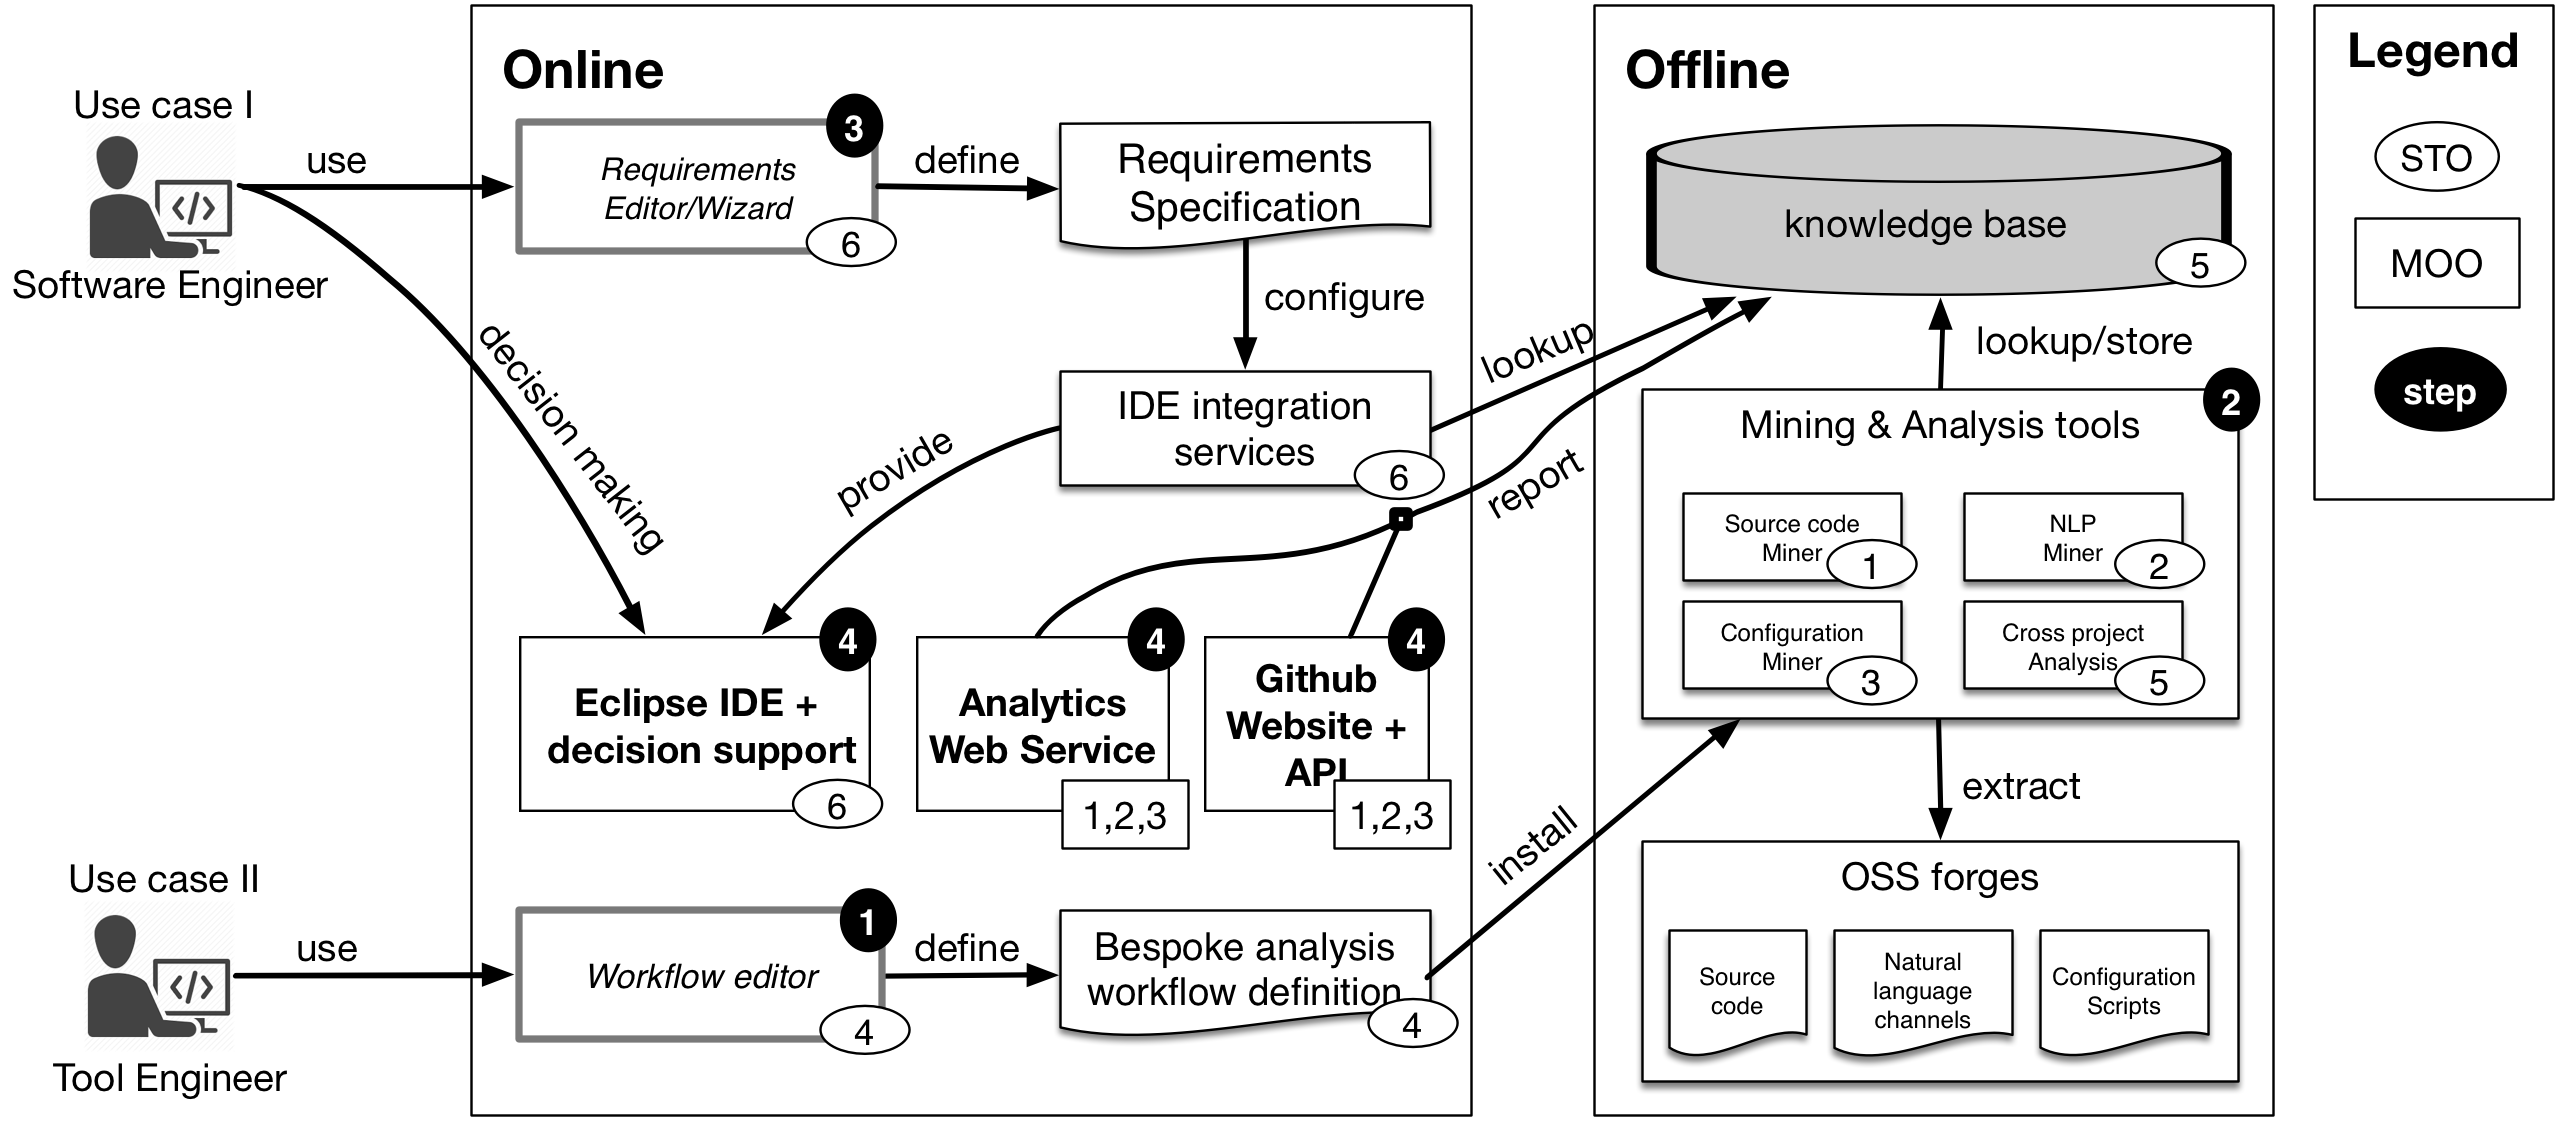
\includegraphics[width=0.9\textwidth]{images/crossminer.png}
	\centering
	\caption{The CROSSMINER Architecture}
	\label{fig:CrossminerApproach}
\end{figure}

\CROSSMINER can be seen as a recommendation system aimed at supporting developers while producing new software by integrating existing open source components. Figure \ref{fig:CrossminerApproach} shows \CROSSMINER at a glance and how the project aims at reaching its objectives. Essentially, the \textit{data preprocessing} challenge is addressed by the \CROSSMINER components contained in the \texttt{Offline} box shown on the right-hand side of Figure~\ref{fig:CrossminerApproach}. The developer context is captured by the IDE (see the \texttt{Online} box in Figure~\ref{fig:CrossminerApproach}), which also produces recommendations that do not require particular and expensive data analysis. For more elaborated recommendations, preprocessed data available in the \texttt{Knowledge Base} is used. Both the IDE and Web based dashboards will be used to present the produced recommendations to the developer. 

%\section{Research Objectives}
%, with the aim of compare the results of new tool by CROSSMINER development team: \CrossSim (Cross Project Relationships for Computing Open Source Software Similarity). \CrossSim is an approach that makes use of graphs for rep-resenting different kinds of relationships in the OSS ecosystem. In particular, with the adoption of the graph representation, we are able to transform the relationships among non-human artifacts, e.g. API utilizations, source code, interactions, and humans, e.g. developers into a mathematically computable format, i.e. one that facilitates various types of computation techniques. Naturally this kind of approaches has to be evaluated, and confronted with others similar tools. My work helps addressing this challenge providing these two tools and evaluating all the results to show how nice is \CrossSim. The main objectives of this thesis are as follows:

\section{Problem Statement}

The work presented in this thesis is coherently related to the \projectName project and it is dedicated to the problem of recommending similar OSS projects for a given project. We perform a performance evaluation of four software similarity tools, namely \MUDABlue \cite{10.1109/APSEC.2004.69}, \CLAN \cite{McMillan:2012:DSS:2337223.2337267}, \RepoPal \cite{10.1109/SANER.2017.7884605}, and \CrossSim \cite{NDRDSEAA2018} to see how well they perform under certain conditions. In this sense, the main research issues that we address in this work are as follows:

\begin{itemize}
	\item Introduce some state-of-the-art approaches for computing software similarity.	
	\item Re-implement four tools for calculating similarities among OSS projects.
	\item Compare the performance of the tools using a set of Java projects collected from GitHub. %CrossSim with three state-of-the-art tools for software similarity measurement. %a comprehensive evaluation of the tools 	
\end{itemize}

\section{Thesis Structure}

The thesis is organized in the following chapters:

\begin{itemize}
	\item Chapter~\ref{sec:MathsBackground} provides a mathematical background related to computing software similarities.
	\item Some of the most notable approaches for computing software similarity are recalled in Chapter~\ref{sec:LiteratureReview}.
	\item Chapter~\ref{sec:Implementation} provides a detailed description of the similarity tools, \ie \MUDABlue \cite{10.1109/APSEC.2004.69}, \CLAN \cite{McMillan:2012:DSS:2337223.2337267}, \RepoPal \cite{10.1109/SANER.2017.7884605}, and \CrossSim \cite{NDRDSEAA2018}.
	\item Chapter~\ref{sec:Evaluation} presents the evaluation and the experimental results.
	\item Finally, Chapter~\ref{sec:Conclusions} sketches out future work and concludes the thesis. 
\end{itemize}